\subsection{研究路线与数据来源}


距今$2000$年前,在人类干预较低的时期,尽管已获“黄河”之名,但这条中华民族的母亲河相较当今仍处于非常原始的状态(图\ref{fig:ch3_why_regime_shift}~A)。
Xu等人(2003)\cite{xu2003a}指出,当时黄河输沙量约为$0.1\sim0.2 Gt$,仅是20世纪均值的十分之一;Chen等人的研究(2012)\cite{chen2012}与王渭泾(2009)\cite{WangWeiJing2009}的著作也指出,黄河河道彼时正处于长时间较平稳的状态,决溢灾害、治河活动也相对较少。
但在20世纪以降,黄河流域几乎已成为学界公认的、是由人类影响主导水循环模式的典型代表,其人-水关系模式被总结为“行洪输沙、生态环境、社会经济”并重综合的复杂系统\cite{jiang2020b}。
因此,与寻找“人类世”的起点有异曲同工之妙,本章研究将假设历史时期人水关系的与近期(百年尺度)是不同的,设计方法在千年尺度上定量识别黄河人-水关系的稳态转换,并分析稳态转换前的人水关系模式。

具体来说,本章研究重点包括以下两个:
(1)识别黄河流域在历史时期内典型稳态转换的发生过程(图\ref{fig:ch3_why_regime_shift}~B)。
稳态转换的发生以“不可逆的大规模结构重组”的发生为标志,而在千年时间尺度上,气候多呈现周期波动的趋势,人类活动的影响总体呈持续增加趋势,且人口、治理、土地利用等变化大多是非线性的\cite{GeQuanSheng2011}。
因此,识别人-水关系稳态转换的关键是将气候的周期性变化、日益增长的人类活动压力各自对流域系统的影响相剥离,并识别人类活动驱动因素超越气候周期波动影响的时期。

(2)分析在该稳态转换发生前,黄河流域人水关系的模式(图\ref{fig:ch3_why_regime_shift}~C)。
根据本研究在\ref{ch2:definitions}\nameref{ch2:definitions}中所下的定义,对人水关系模式的总结需要考虑“决定社会-水文循环的利益相关者是谁”,以及“该利益相关者的认知或行动模式是怎样的”等问题。
由于历史时期可获取的数据或记载的局限性,研究中将利益相关者简单分为“中央政府”与“大众”,其影响社会-水文过程的主要因素分别是对河流的治理,以及对土地利用-覆被的改造。
因此,总结此时期人-水关系的关键,是在千年时间尺度下分析上述因素是否对社会-水文反馈循环产生明显影响。

\begin{figure}[H] % use float package if you want it here
    \centering
    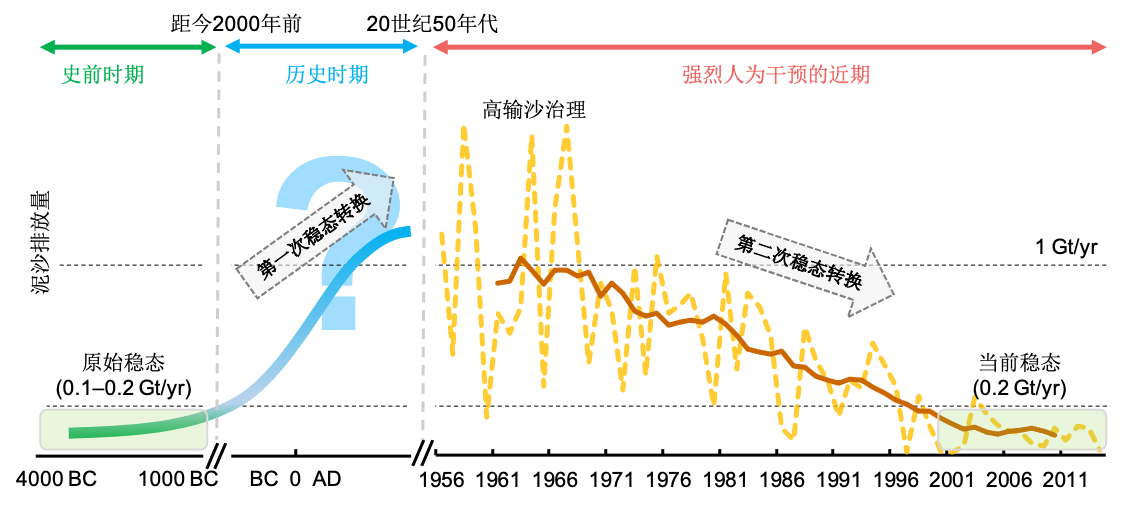
\includegraphics[width=\textwidth]{img/ch3/ch3_why_regime_shift.png}
    \caption[黄河流域千年尺度人-水关系变化的关键研究问题]{黄河流域千年尺度人-水关系变化的关键研究问题。第一次稳态转换发生在历史时期}
    \label{fig:ch3_why_regime_shift}
\end{figure}

此外,数据是开展历史时期研究的主要挑战,上述研究路线须根据可获得的、质量可靠的数据来设计具体方法和指标。本研究通过整理前人在沉积学、气候学、历史学等领域的著述,获取到公开发表、质量可靠的数据及其来源如表\ref{tab:data_source}所示。

% Table generated by Excel2LaTeX from sheet 'Sheet1'
\begin{table}[hbt]
  % \centering
  % \begin{minipage}[t]{0.8\linewidth}
  \caption[千年尺度黄河稳态转换识别的数据来源]{千年尺度黄河稳态转换识别的数据来源。}
    % \begin{tabular}{llllll}
    \begin{tabularx}{\textwidth}{ p{2cm} L p{5cm} L p{3cm} L}
    \toprule
    数据集   & 类型    & 描述    & 原始材料  & 可信度   & 参考 \\
    \midrule
    干旱和洪涝频率 & 气候驱动力 & 每五十年为一个时期,分别统计中原、华北平原地区的干旱、洪涝灾害的频次 & 官方和地方的史料记录 & 根据历史材料的丰富程度,在不同时期的可信度是不一致的 & 葛全胜,2011 \cite{GeQuanSheng2011} \\
    湿润指数累计距平 & 气候驱动力 & 根据史料中与湿度相关的记录,评估历史时期气候湿润程度的等级 & 官方和地方的史料记录 & 根据历史材料的丰富程度,在不同时期的可信度是不一致的 & Zheng,2006 \cite{zheng2006} \\
    黄河中游人口数量 & 人类活动驱动力 & 利用史料记录推断的黄河中游人口 & 历史户籍注册信息 & 数字不精确但可以反映趋势以供纵向比较 & Chen et al., 2012 \cite{chen2012} \\
    农牧交错带的北界位置 & 混合驱动力 & 农牧交界线距离潼关所在维度的平均距离 & 中国历史地图集 & 时间采样点比较少,但每个点的位置数据较为可信 & 谭其骧,1996 \cite{TanQiXiang1996} \\
    三门峡峡谷航运数据 & 影响$^*$    & 三门峡航运通行难易程度的等级 & 官方和地方的史料记录 & 数据从可靠的史料来源获得,但存在数据缺失情况 & 王守春,1993 \cite{WangShouChun1993} \\ %TODO 这里还需要参考,查证王老师那的书
    黄河下游决溢数据 & 影响    & 黄河下游堤防崩溃的次数 & 官方和地方的史料记录 & 根据历史材料的丰富程度,在不同时期的可信度是不一致的 & Chen et al., 2012 \cite{chen2012} \\
    黄河古河道沉积速率 & 影响    & 结合历史地图和取样测定的黄河古河道沉积速率 & 沉积样本  & 样本所在的古河道时间跨度越长样本越精确 & Xu 2003 \cite{xu2003a} \\
    \bottomrule
    % \end{tabular}%
  \end{tabularx}\\[2pt]
  % \leftalighn
  \footnotesize 注:*影响:指黄河关键特征变化带来的影响。\\\label{tab:data_source}%
  % \end{minipage}
\end{table}%



\subsection{稳态转换过程的识别途径}

在历史时期的黄河流域,由于缺乏对流域的系统性认识,不断增长的人为压力带来的影响主要是中游黄土区的开垦进而导致输沙量的提升\cite{wu2020a}。
针对此次稳态转换的特点,分析其发生过程的关键是识别黄河输沙量的变化与气候周期“脱钩”的时段,因此本研究设计了如图\ref{fig:ch3_regime_shift_detect}所示的稳态转换识别框架。
周期性气候变化和不断增长的人为因素(主要是中游易侵蚀区的粮食生产)共同驱动着产沙量、产水量两个关键特征的变化,二者的变化则会在流域内触发一系列影响因素变化。
在气候湿润时期,土壤侵蚀和径流增加了更丰富的降水,会导致产水量和产沙量同时增增加,因此二者也存在一定的正相关关系。
但而随着人类活动压力增大,开垦造成粮食产量增通常减少植被的覆盖范围,从而加剧水土流失,这主要导致产沙量增多。
因此通过分析与产沙过程、产水过程关系有所差异的三类影响因素变化趋势(图\ref{fig:ch3_impacts}),理论上可以找到“产沙量增加比产水量增加更显著”的关键变化时期。

% 总体潮湿的气候让宋代农牧交错带北移,但极端气候增多,干旱造就了土地退化,洪水增加了侵蚀,平水年份水量较多。
% 清朝乾隆之后航运断绝,平水时期的三门峡河道都难以行船了,这或许是明清黄河输沙持续恶化的体现。
% 由于直接证据的缺乏,河道兴废、三角洲扩张,结合决溢材料,三者结合起来才能说明河道的沉沙情况。

\begin{figure}[H] % use float package if you want it here
    \centering
    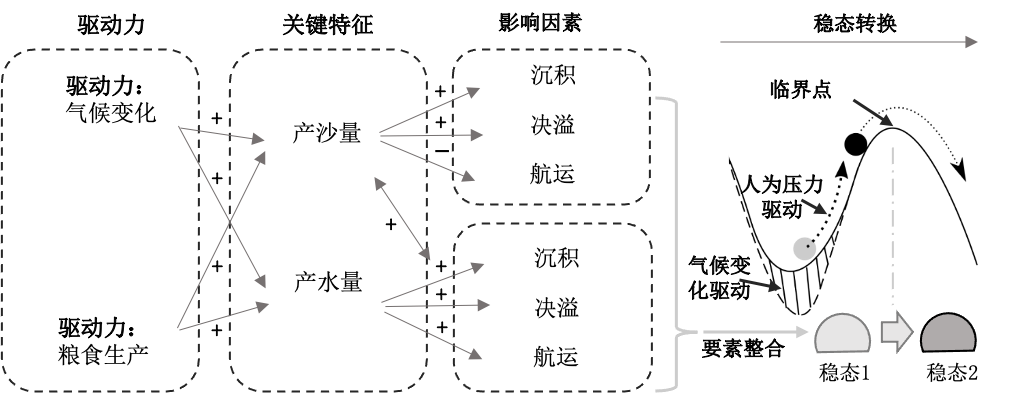
\includegraphics{ch3/ch3_workflow.png}
    \caption[黄河历史时期稳态转换识别的框架]{黄河历史时期稳态转换识别的框架。气候变化和粮食生产是致使稳态转换发生的潜在驱动力;稳态转换发生时影响的关键是产沙量和产水量;二者的变化又会触发流域一系列影响因素变化。灰色箭头及其旁边的符号表示消极或者积极的影响路径;在驱动力推动系统接近临界点时,所有受影响因素经整合后会展示稳态转换是否发生。}
    \label{fig:ch3_regime_shift_detect}
\end{figure}

\begin{figure}[H] % use float package if you want it here
    \centering
    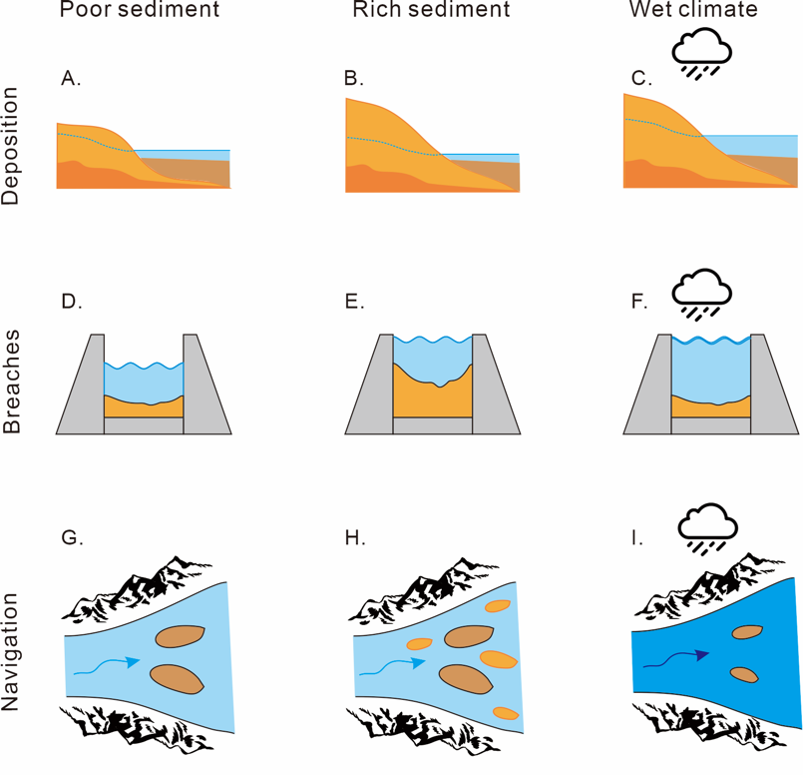
\includegraphics{img/ch3/ch3_impacts.png}
    \caption[黄河历史产水量和产沙量带来的影响]{黄河历史产水量和产沙量带来的影响。输沙和产水两个主要特征分别对沉积(A-C);决溢(D-F);航运(G-H)的影响。
    (1)对于沉积数据,产沙量高(从A到B)可能导致下游沉积速率增加\cite{xu2003a};
    (2)对于洪泛数据,产沙量高(从D到E)或者气候湿润期(从D到F)都有可能导致更多的决溢洪泛\cite{chen2012};
    (3)对于航运数据,产沙量高(从G到H)会增加浅滩数量,从而使航运变得更加困难,而潮湿的气候时期由于平均径流量变大,三门峡的通航将更加容易\cite{WangShouChun1993}。}
    \label{fig:ch3_impacts}
\end{figure}

用以分析稳态转换驱动因素的数据集匹配本研究需要,均不做进一步处理,而反映黄河特征变化带来的影响的三个数据集(黄河古河道沉积速率、洪泛决溢次数、三门峡航运情况)按表\ref{tab:ch3_impacts_magnitude}进行半定量化。
此外,由于历史资料难以避免具有不确定性,需依据上述三个数据集各自特点评估其置信度并进行整合。
我们先分别对沉积、决溢、航运三个数据集各自的置信度按公式\ref{eq:ch3_credibility}所示方法进行估计:
(1)由于沉积每个数据是对遗留河床样本的平均估计,遗留时间越长的古河床样本所估计值相对可靠;
(2)溃堤数据的置信度取决于官方史料的可靠程度,该时期的历史记录更可靠、存留的历史记录更多,则该时期的估计值也更可靠;
(3)航运数据出处未给出各时段的史料置信度,所以该数据的置信情况使用时段内航运相关记录的数量进行评估。
最后,再将每个数据集置信度按极大-极小归一化(公式\ref{eq:ch3_normalize})后同样划分为三个置信等级。

% Table generated by Excel2LaTeX from sheet '影响强度半定量化'
\begin{table}[!htbp]
    \caption{黄河关键特征变化影响强度的半定量分级}
      \begin{tabularx}{\textwidth}{p{1.5cm} LLL}
      \toprule
      \multicolumn{1}{l}{强度等级} & 古河道沉积速率 & 洪泛决溢频次 & 三门峡航运情况 \\
      \midrule
      1     & $0 \sim 2$ cm/yr & < 10次 / 20yrs & 自由通行 \\
      2     & $2 \sim 4$ cm/yr & 10~20次 / 20yrs & 需要人力辅助 \\
      3     & $\> 4cm/yr$ & >20次 / 20yrs & 完全无法通行 \\
      \bottomrule
      \end{tabularx}%
    \label{tab:ch3_impacts_magnitude}%
\end{table}%


\begin{equation}
    \label{eq:ch3_credibility}
    Credibility_X = 
    \left\{\begin{array}{l}
        \text{[沉积, ]} 1 / \frac{1}{n} \sum_{i=1}^n T_i\\
        \text{[决溢, ]} \prod_{i=1}^n C_i\\
        \text{[航运, ]} N_i
    \end{array}\right.
\end{equation}

其中$n$均为给定时段内各数据集样本/记录的数量。$T_i$为每个沉积样本所在古河道的时间跨度;$C_i$是每个历史记录所在时段的置信程度(由数据作者给出的评估,详见表\ref{tab:data_source});$N_i$是每个时期航运相关历史记录的数量。

\begin{equation}
    \label{eq:ch3_normalize}
    C_{nom}=\frac{C-C_{\min}}{C_{\max}-C_{\min}}
\end{equation}

其中$C_{X}$为参照公式\ref{eq:ch3_credibility}对数据集$X$进行评估后的置信程度,$C_{\min, X}$, $C_{\max, X}$分别为数据的最小值和最大值。$C_nom$为归一化后的置信程度。

\subsection{稳态转换识别指标构建}

\subsection{人水关系反馈回路识别}
% 以及缺乏系统性地“只关注河道”的河流治理模式\cite{WangWeiJing2009}